\documentclass[]{article}
\usepackage{graphicx}
\usepackage{listings}

%opening
\title{Tarea 1}
\author{Rivera Plascencia Bryan 2BM2}

\begin{document}

\maketitle

\begin{abstract}

\end{abstract}
\newpage
\section{¿Que es ordenamiento?}
Es la operación de arreglar los elementos de algún orden secuencial de acuerdo a un criterio de ordenamiento.

\section{Quicksort}

\subsection{Funcionamiento}
Elige un elemento del conjunto de elementos a ordenar, el cual se le puede llamar pivote.\\
Debemos acomodar los demás elementos de la lista a cada lado del pivote, de manera que a un lado queden todos los menores que él y al otro los mayores.\\
La lista queda separada en dos sublistas, formadas por los elementos de la izquierda del pivote y otra por los que están a la derecha del pivote.\\
Después debemos de repetir este proceso de forma recursiva para cada sublista mientras estas contengan mas de un elemento.\\
Cuando se termine este procedimiento los elementos de la lista estarán ordenados.\\


\subsection{Código}
\begin{lstlisting}[language=C]
#include <stdio.h>

void swap(int* a, int* b) {
	int t = *a;
	*a = *b;
	*b = t;
}
int partition(int arr[], int low, int high) {
	int pivot = arr[high]; // Tomar el ultimo elemento como pivote
	int i = (low - 1); // El indice del elemento mas pequeno

	for (int j = low; j <= high - 1; j++) {
		// Si el elemento actual es menor o igual al pivote
		if (arr[j] <= pivot) {
			i++; // Incrementar el indice del elemento mas pequeno
			swap(&arr[i], &arr[j]);
		}
	}
	swap(&arr[i + 1], &arr[high]);
	return (i + 1);
}

void quickSort(int arr[], int low, int high) {
	if (low < high) {

		// Encuentra el indice de particion
		int pi = partition(arr, low, high);

		// Ordena los elementos antes y despues de la particion
		quickSort(arr, low, pi - 1);
		quickSort(arr, pi + 1, high);
	}
}

int main() {
	int arr[] = {64, 25, 12, 22, 11};
	int n = sizeof(arr) / sizeof(arr[0]);  
	printf("Arreglo original: ");
	for (int i = 0; i < n; i++) {
		printf("%d ", arr[i]);
	}

	quickSort(arr, 0, n - 1);
	printf("\nArreglo ordenado: ");
	for (int i = 0; i < n; i++) {
		printf("%d ", arr[i]);
	}

	return 0;
}

\end{lstlisting}
\subsection{Complejidad}
En el mejor de los casos, el pivote termina en el centro de la lista, dividiéndola en dos sublistas de igual tamaño y la complejidad seria de O(n*log n).\\
En el peor de los casos el pivote termina en el extremo de la lista, y el orden de complejidad del algoritmo seria O(n2) , el peor de los casos dependerá de la implementación del algoritmo aunque habitualmente ocurre en listas que se encuentran ordenadas o casi oredenadas.\\
El caso promedio el orden es (n*log n).\\

\subsection{Ventajas:}
Requiere de pocos recursos en comparación a otros métodos de ordenamiento.\\
En la mayoría de los casos, se requiere aproximadamente  de n* log N.\\
Ciclo interno es extremadamente corto.\\
No se requiere de espacio adicional durante la ejecución.\\

\subsection{Desventajas:}
Se complica la implementación si la recursión no es posible.\\
Peor caso, se requiere N2.\\
Un simple error en la implementación puede pasar sin detección, lo que provocaría un rendimiento pésimo.\\
No es útil para aplicaciones de entrada dinámica, donde se requiere reordenar una lista de elementos con nuevos valores.\\
Se pierde el orden relativo de elementos idénticos.\\

\subsection{Aplicaciones:}
Para ordenar una lista de números/nombres.\\
Utilización antes de implementar una búsqueda binaria.\\
Utilizando como método de ordenamiento en tarjetas graficas.\\

\subsection{Ejemplos}

\begin{figure}[h]
	\centering
	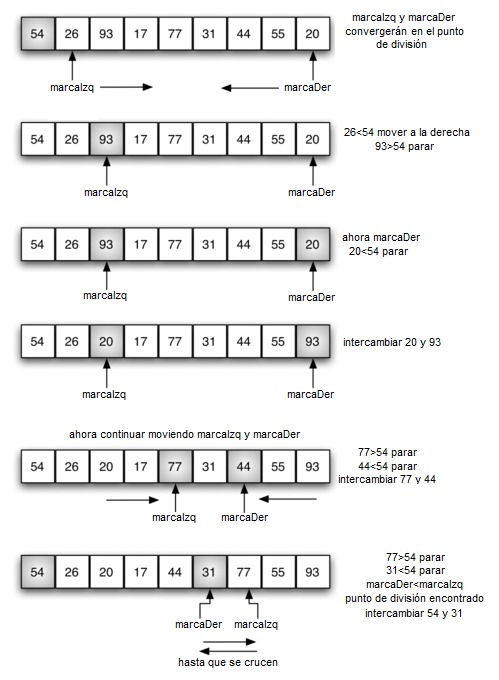
\includegraphics[width=0.6\linewidth]{C:/Users/bryan/Downloads/quick1}
	\caption{}
	\label{fig:quick1}
\end{figure}
\begin{figure}[t!]
	\centering
	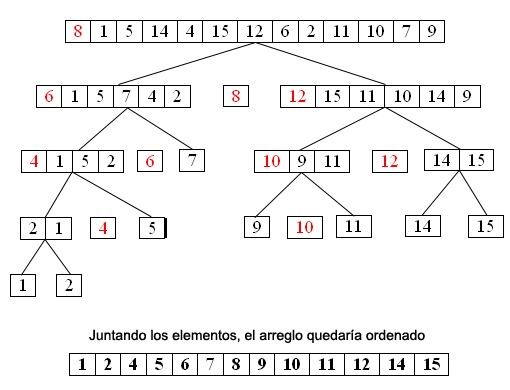
\includegraphics[width=0.7\linewidth]{C:/Users/bryan/Downloads/quick2}
	\caption{}
	\label{fig:quick2}
\end{figure}

\newpage
\section{Mergesort}

\subsection{Funcionamiento}
Debemos de dividir el arreglo por la mitad una y otra vez hasta que cada pieza de tenga un solo elemento de longitud.\\
Luego esos elementos se vuelven a juntar (mezclados) en orden de clasificación.\\
Ahora tenemos que unirlos de nuevo en orden de mezcla; primero fusionamos elementos individuales en pares, cada par se fusiona en orden de mezcla.
Luego fusionamos los pares en orden de mezcla.\\
Y luego fusionamos los dos últimos grupos .\\

\subsection{Código}
\begin{lstlisting}[language=C]
#include <stdio.h>

void merge(int arr[], int l, int m, int r) {
	int i, j, k;
	int n1 = m - l + 1;
	int n2 = r - m;
	
	// Crear arreglos temporales
	int L[n1], R[n2];
	
	// Copiar datos a los arreglos temporales L[] y R[]
	for (i = 0; i < n1; i++)
	L[i] = arr[l + i];
	for (j = 0; j < n2; j++)
	R[j] = arr[m + 1 + j];
	
	// Combinar los arreglos temporales en el arreglo original arr[l..r]
	i = 0; // Indice inicial de primer subarreglo
	j = 0; // Indice inicial de segundo subarreglo
	k = l; // Indice inicial del subarreglo combinado
	while (i < n1 && j < n2) {
		if (L[i] <= R[j]) {
			arr[k] = L[i];
			i++;
		} else {
			arr[k] = R[j];
			j++;
		}
		k++;
	}
	
	// Copiar los elementos restantes de L[], si los hay
	while (i < n1) {
		arr[k] = L[i];
		i++;
		k++;
	}
	
	// Copiar los elementos restantes de R[], si los hay
	while (j < n2) {
		arr[k] = R[j];
		j++;
		k++;
	}
}

void mergeSort(int arr[], int l, int r) {
	if (l < r) {
		// Encuentra el punto medio del arreglo
		int m = l + (r - l) / 2;
		
		// Ordena la primera mitad
		mergeSort(arr, l, m);
		
		// Ordena la segunda mitad
		mergeSort(arr, m + 1, r);
		
		// Combina las dos mitades ordenadas
		merge(arr, l, m, r);
	}
}

int main() {
	int arr[] = {12, 11, 13, 5, 6, 7};
	int arr_size = sizeof(arr) / sizeof(arr[0]);
	
	printf("Arreglo original:\n");
	for (int i = 0; i < arr_size; i++) {
		printf("%d ", arr[i]);
	}
	
	mergeSort(arr, 0, arr_size - 1);
	
	printf("\nArreglo ordenado:\n");
	for (int i = 0; i < arr_size; i++) {
		printf("%d ", arr[i]);
	}
	
	return 0;
}

\end{lstlisting}
\subsection{Complejidad}
La mezcla de dos listados tiene una complejidad lineal O(n+m), donde n+m es la suma del tamaño de ambos listados.\\

\subsection{Ventajas:}
Es un método estable de ordenamiento mientras la operación de mezcla sea implementada correctamente.
Su algoritmo tiene mucha estabilidad (se evitan problemas de intercambio de claves en la manipulación de datos).\\
Es efectivo para conjuntos de datos que se puedan acceder secuencialmente como arreglos, vectores y listas ligadas.\\

\subsection{Desventajas:}
Su principal desventaja radica en que está definido recursivamente y su implementación no recursiva emplea una pila, por lo que requiere un espacio adicional de memoria para almacenarla.\\
A los algoritmos que realizan el proceso de ordenamiento dentro del mismo vector se les denomina algoritmos de ordenamiento “IN-SITU”, el algoritmo de mergesort no pertenece a esta familia ya que no utiliza el espacio sobe el que están almacenados los datos sino que para poder funcionar requiere de un espacio de memoria adicional del tamaño de los datos a ordenar en el cual se realicen las mezclas.\\
\newpage
\subsection{Ejemplos}
\begin{figure}[h!]
	\centering
	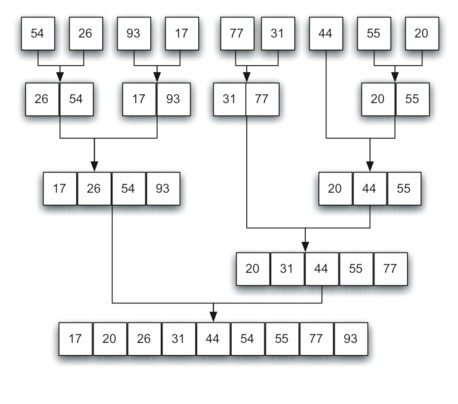
\includegraphics[width=0.7\linewidth]{C:/Users/bryan/Downloads/merge1}
	\caption{}
	\label{fig:merge1}
\end{figure}
\begin{figure}[t!]
	\centering
	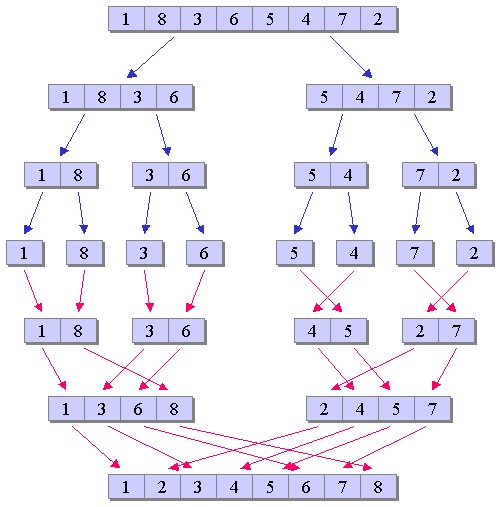
\includegraphics[width=0.7\linewidth]{C:/Users/bryan/Downloads/merge2}
	\caption{}
	\label{fig:merge2}
\end{figure}
\newpage
\section{Bibliografia}

\underline{\textbf{https://es.wikipedia.org/wiki/Quicksort}}\\
\underline{\textbf{https://quicksortweb.wordpress.com/2017/10/07/ventajas-desventajas-y-aplicaciones/}}\\
\underline{\textbf{https://runestone.academy/ns/books/published/pythoned/SortSearch/ElOrdenamientoRapido.html}}\\
\underline{\textbf{https://ronnyml.wordpress.com/2009/07/19/quicksort-en-c/}}\\
\underline{\textbf{https://es.wikipedia.org/wiki/Ordenamiento\_por\_mezcla}}\\
\underline{\textbf{https://platzi.com/tutoriales/1469-algoritmos-practico/4260-merge-sort-en-java/}}\\
\underline{\textbf{https://binarycoffee.dev/post/conociendo-el-ordenamiento-por-mezcla-merge-sort}}\\


\end{document}
